\documentclass[1p]{elsarticle_modified}
%\bibliographystyle{elsarticle-num}

%\usepackage[colorlinks]{hyperref}
%\usepackage{abbrmath_seonhwa} %\Abb, \Ascr, \Acal ,\Abf, \Afrak
\usepackage{amsfonts}
\usepackage{amssymb}
\usepackage{amsmath}
\usepackage{amsthm}
\usepackage{scalefnt}
\usepackage{amsbsy}
\usepackage{kotex}
\usepackage{caption}
\usepackage{subfig}
\usepackage{color}
\usepackage{graphicx}
\usepackage{xcolor} %% white, black, red, green, blue, cyan, magenta, yellow
\usepackage{float}
\usepackage{setspace}
\usepackage{hyperref}

\usepackage{tikz}
\usetikzlibrary{arrows}

\usepackage{multirow}
\usepackage{array} % fixed length table
\usepackage{hhline}

%%%%%%%%%%%%%%%%%%%%%
\makeatletter
\renewcommand*\env@matrix[1][\arraystretch]{%
	\edef\arraystretch{#1}%
	\hskip -\arraycolsep
	\let\@ifnextchar\new@ifnextchar
	\array{*\c@MaxMatrixCols c}}
\makeatother %https://tex.stackexchange.com/questions/14071/how-can-i-increase-the-line-spacing-in-a-matrix
%%%%%%%%%%%%%%%

\usepackage[normalem]{ulem}

\newcommand{\msout}[1]{\ifmmode\text{\sout{\ensuremath{#1}}}\else\sout{#1}\fi}
%SOURCE: \msout is \stkout macro in https://tex.stackexchange.com/questions/20609/strikeout-in-math-mode

\newcommand{\cancel}[1]{
	\ifmmode
	{\color{red}\msout{#1}}
	\else
	{\color{red}\sout{#1}}
	\fi
}

\newcommand{\add}[1]{
	{\color{blue}\uwave{#1}}
}

\newcommand{\replace}[2]{
	\ifmmode
	{\color{red}\msout{#1}}{\color{blue}\uwave{#2}}
	\else
	{\color{red}\sout{#1}}{\color{blue}\uwave{#2}}
	\fi
}

\newcommand{\Sol}{\mathcal{S}} %segment
\newcommand{\D}{D} %diagram
\newcommand{\A}{\mathcal{A}} %arc


%%%%%%%%%%%%%%%%%%%%%%%%%%%%%5 test

\def\sl{\operatorname{\textup{SL}}(2,\Cbb)}
\def\psl{\operatorname{\textup{PSL}}(2,\Cbb)}
\def\quan{\mkern 1mu \triangleright \mkern 1mu}

\theoremstyle{definition}
\newtheorem{thm}{Theorem}[section]
\newtheorem{prop}[thm]{Proposition}
\newtheorem{lem}[thm]{Lemma}
\newtheorem{ques}[thm]{Question}
\newtheorem{cor}[thm]{Corollary}
\newtheorem{defn}[thm]{Definition}
\newtheorem{exam}[thm]{Example}
\newtheorem{rmk}[thm]{Remark}
\newtheorem{alg}[thm]{Algorithm}

\newcommand{\I}{\sqrt{-1}}
\begin{document}

%\begin{frontmatter}
%
%\title{Boundary parabolic representations of knots up to 8 crossings}
%
%%% Group authors per affiliation:
%\author{Yunhi Cho} 
%\address{Department of Mathematics, University of Seoul, Seoul, Korea}
%\ead{yhcho@uos.ac.kr}
%
%
%\author{Seonhwa Kim} %\fnref{s_kim}}
%\address{Center for Geometry and Physics, Institute for Basic Science, Pohang, 37673, Korea}
%\ead{ryeona17@ibs.re.kr}
%
%\author{Hyuk Kim}
%\address{Department of Mathematical Sciences, Seoul National University, Seoul 08826, Korea}
%\ead{hyukkim@snu.ac.kr}
%
%\author{Seokbeom Yoon}
%\address{Department of Mathematical Sciences, Seoul National University, Seoul, 08826,  Korea}
%\ead{sbyoon15@snu.ac.kr}
%
%\begin{abstract}
%We find all boundary parabolic representation of knots up to 8 crossings.
%
%\end{abstract}
%\begin{keyword}
%    \MSC[2010] 57M25 
%\end{keyword}
%
%\end{frontmatter}

%\linenumbers
%\tableofcontents
%
\newcommand\colored[1]{\textcolor{white}{\rule[-0.35ex]{0.8em}{1.4ex}}\kern-0.8em\color{red} #1}%
%\newcommand\colored[1]{\textcolor{white}{ #1}\kern-2.17ex	\textcolor{white}{ #1}\kern-1.81ex	\textcolor{white}{ #1}\kern-2.15ex\color{red}#1	}

{\Large $\underline{12n_{0277}~(K12n_{0277})}$}

\setlength{\tabcolsep}{10pt}
\renewcommand{\arraystretch}{1.6}
\vspace{1cm}\begin{tabular}{m{100pt}>{\centering\arraybackslash}m{274pt}}
\multirow{5}{120pt}{
	\centering
	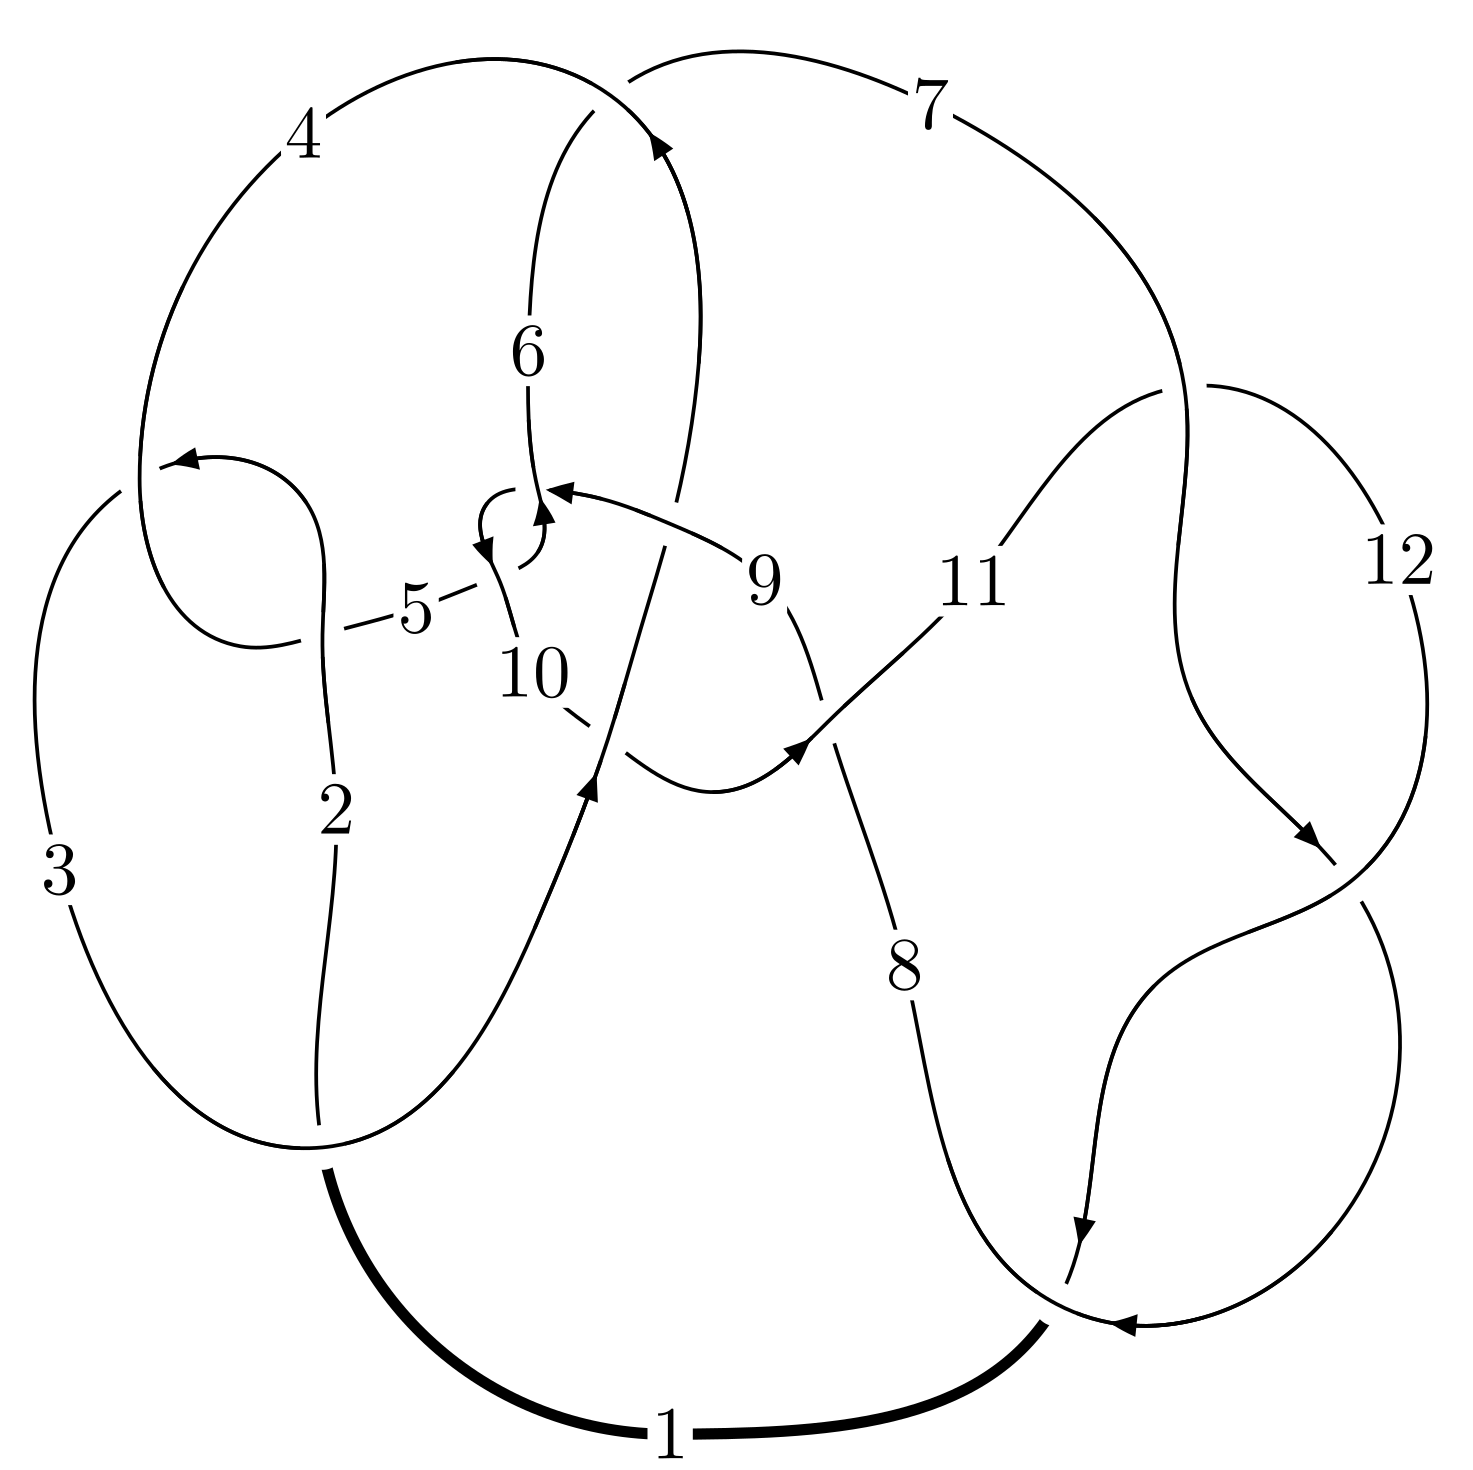
\includegraphics[width=112pt]{../../../GIT/diagram.site/Diagrams/png/2366_12n_0277.png}\\
\ \ \ A knot diagram\footnotemark}&
\allowdisplaybreaks
\textbf{Linearized knot diagam} \\
\cline{2-2}
 &
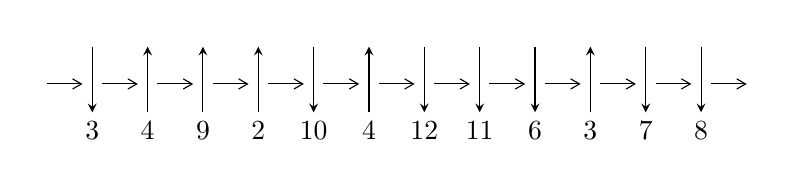
\begin{tikzpicture}[x=20pt, y=17pt]
	% nodes
	\node (C0) at (0, 0) {};
	\node (C1) at (1, 0) {};
	\node (C1U) at (1, +1) {};
	\node (C1D) at (1, -1) {3};

	\node (C2) at (2, 0) {};
	\node (C2U) at (2, +1) {};
	\node (C2D) at (2, -1) {4};

	\node (C3) at (3, 0) {};
	\node (C3U) at (3, +1) {};
	\node (C3D) at (3, -1) {9};

	\node (C4) at (4, 0) {};
	\node (C4U) at (4, +1) {};
	\node (C4D) at (4, -1) {2};

	\node (C5) at (5, 0) {};
	\node (C5U) at (5, +1) {};
	\node (C5D) at (5, -1) {10};

	\node (C6) at (6, 0) {};
	\node (C6U) at (6, +1) {};
	\node (C6D) at (6, -1) {4};

	\node (C7) at (7, 0) {};
	\node (C7U) at (7, +1) {};
	\node (C7D) at (7, -1) {12};

	\node (C8) at (8, 0) {};
	\node (C8U) at (8, +1) {};
	\node (C8D) at (8, -1) {11};

	\node (C9) at (9, 0) {};
	\node (C9U) at (9, +1) {};
	\node (C9D) at (9, -1) {6};

	\node (C10) at (10, 0) {};
	\node (C10U) at (10, +1) {};
	\node (C10D) at (10, -1) {3};

	\node (C11) at (11, 0) {};
	\node (C11U) at (11, +1) {};
	\node (C11D) at (11, -1) {7};

	\node (C12) at (12, 0) {};
	\node (C12U) at (12, +1) {};
	\node (C12D) at (12, -1) {8};
	\node (C13) at (13, 0) {};

	% arrows
	\draw[->,>={angle 60}]
	(C0) edge (C1) (C1) edge (C2) (C2) edge (C3) (C3) edge (C4) (C4) edge (C5) (C5) edge (C6) (C6) edge (C7) (C7) edge (C8) (C8) edge (C9) (C9) edge (C10) (C10) edge (C11) (C11) edge (C12) (C12) edge (C13) ;	\draw[->,>=stealth]
	(C1U) edge (C1D) (C2D) edge (C2U) (C3D) edge (C3U) (C4D) edge (C4U) (C5U) edge (C5D) (C6D) edge (C6U) (C7U) edge (C7D) (C8U) edge (C8D) (C9U) edge (C9D) (C10D) edge (C10U) (C11U) edge (C11D) (C12U) edge (C12D) ;
	\end{tikzpicture} \\
\hhline{~~} \\& 
\textbf{Solving Sequence} \\ \cline{2-2} 
 &
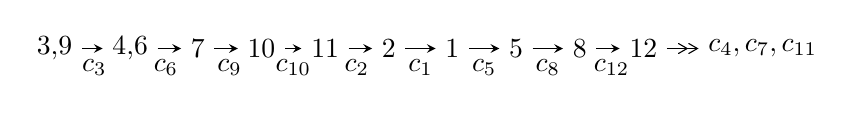
\begin{tikzpicture}[x=23pt, y=7pt]
	% node
	\node (A0) at (-1/8, 0) {3,9};
	\node (A1) at (17/16, 0) {4,6};
	\node (A2) at (17/8, 0) {7};
	\node (A3) at (25/8, 0) {10};
	\node (A4) at (33/8, 0) {11};
	\node (A5) at (41/8, 0) {2};
	\node (A6) at (49/8, 0) {1};
	\node (A7) at (57/8, 0) {5};
	\node (A8) at (65/8, 0) {8};
	\node (A9) at (73/8, 0) {12};
	\node (C1) at (1/2, -1) {$c_{3}$};
	\node (C2) at (13/8, -1) {$c_{6}$};
	\node (C3) at (21/8, -1) {$c_{9}$};
	\node (C4) at (29/8, -1) {$c_{10}$};
	\node (C5) at (37/8, -1) {$c_{2}$};
	\node (C6) at (45/8, -1) {$c_{1}$};
	\node (C7) at (53/8, -1) {$c_{5}$};
	\node (C8) at (61/8, -1) {$c_{8}$};
	\node (C9) at (69/8, -1) {$c_{12}$};
	\node (A10) at (11, 0) {$c_{4},c_{7},c_{11}$};

	% edge
	\draw[->,>=stealth]	
	(A0) edge (A1) (A1) edge (A2) (A2) edge (A3) (A3) edge (A4) (A4) edge (A5) (A5) edge (A6) (A6) edge (A7) (A7) edge (A8) (A8) edge (A9) ;
	\draw[->>,>={angle 60}]	
	(A9) edge (A10);
\end{tikzpicture} \\ 

\end{tabular} \\

\footnotetext{
The image of knot diagram is generated by the software ``\textbf{Draw programme}" developed by Andrew Bartholomew(\url{http://www.layer8.co.uk/maths/draw/index.htm\#Running-draw}), where we modified some parts for our purpose(\url{https://github.com/CATsTAILs/LinksPainter}).
}\phantom \\ \newline 
\centering \textbf{Ideals for irreducible components\footnotemark of $X_{\text{par}}$} 
 
\begin{align*}
I^u_{1}&=\langle 
-1.31866\times10^{31} u^{44}-1.02208\times10^{31} u^{43}+\cdots+1.69549\times10^{31} b+1.38177\times10^{31},\\
\phantom{I^u_{1}}&\phantom{= \langle  }5.31714\times10^{31} u^{44}+5.34083\times10^{31} u^{43}+\cdots+4.23874\times10^{31} a-8.50686\times10^{31},\;u^{45}+u^{44}+\cdots-3 u+5\rangle \\
I^u_{2}&=\langle 
u^3 b^2+6 b^2 u^2-2 u^3 b+b^3- b^2 u-4 u^3-3 b^2-2 b u-6 u^2-9 b+3 u+3,\;- u^2+a,\;u^4- u^2+1\rangle \\
\\
\end{align*}
\raggedright * 2 irreducible components of $\dim_{\mathbb{C}}=0$, with total 57 representations.\\
\footnotetext{All coefficients of polynomials are rational numbers. But the coefficients are sometimes approximated in decimal forms when there is not enough margin.}
\newpage
\renewcommand{\arraystretch}{1}
\centering \section*{I. $I^u_{1}= \langle -1.32\times10^{31} u^{44}-1.02\times10^{31} u^{43}+\cdots+1.70\times10^{31} b+1.38\times10^{31},\;5.32\times10^{31} u^{44}+5.34\times10^{31} u^{43}+\cdots+4.24\times10^{31} a-8.51\times10^{31},\;u^{45}+u^{44}+\cdots-3 u+5 \rangle$}
\flushleft \textbf{(i) Arc colorings}\\
\begin{tabular}{m{7pt} m{180pt} m{7pt} m{180pt} }
\flushright $a_{3}=$&$\begin{pmatrix}1\\0\end{pmatrix}$ \\
\flushright $a_{9}=$&$\begin{pmatrix}0\\u\end{pmatrix}$ \\
\flushright $a_{4}=$&$\begin{pmatrix}1\\- u^2\end{pmatrix}$ \\
\flushright $a_{6}=$&$\begin{pmatrix}-1.25442 u^{44}-1.26001 u^{43}+\cdots+17.1020 u+2.00693\\0.777745 u^{44}+0.602821 u^{43}+\cdots-13.4579 u-0.814966\end{pmatrix}$ \\
\flushright $a_{7}=$&$\begin{pmatrix}-0.857487 u^{44}-0.977954 u^{43}+\cdots+9.89939 u+1.21992\\0.622066 u^{44}+0.528291 u^{43}+\cdots-11.1287 u-1.38935\end{pmatrix}$ \\
\flushright $a_{10}=$&$\begin{pmatrix}-0.251178 u^{44}-0.450479 u^{43}+\cdots+8.17819 u+4.56451\\-0.0401479 u^{44}-0.367454 u^{43}+\cdots-2.48738 u+6.40126\end{pmatrix}$ \\
\flushright $a_{11}=$&$\begin{pmatrix}-0.291326 u^{44}-0.817933 u^{43}+\cdots+5.69081 u+10.9658\\-0.0401479 u^{44}-0.367454 u^{43}+\cdots-2.48738 u+6.40126\end{pmatrix}$ \\
\flushright $a_{2}=$&$\begin{pmatrix}- u^2+1\\u^4\end{pmatrix}$ \\
\flushright $a_{1}=$&$\begin{pmatrix}u^4- u^2+1\\u^4\end{pmatrix}$ \\
\flushright $a_{5}=$&$\begin{pmatrix}u^4- u^2+1\\- u^6- u^2\end{pmatrix}$ \\
\flushright $a_{8}=$&$\begin{pmatrix}-0.701040 u^{44}-1.41736 u^{43}+\cdots+4.97925 u+12.1312\\-0.302362 u^{44}-0.273729 u^{43}+\cdots+1.07283 u-1.67880\end{pmatrix}$ \\
\flushright $a_{12}=$&$\begin{pmatrix}-1.08462 u^{44}-1.85577 u^{43}+\cdots+9.70163 u+13.7283\\0.284549 u^{44}+0.197516 u^{43}+\cdots-7.73043 u-0.550539\end{pmatrix}$\\&\end{tabular}
\flushleft \textbf{(ii) Obstruction class $= -1$}\\~\\
\flushleft \textbf{(iii) Cusp Shapes $= -0.476359 u^{44}-0.619053 u^{43}+\cdots+0.718999 u+7.19239$}\\~\\
\newpage\renewcommand{\arraystretch}{1}
\flushleft \textbf{(iv) u-Polynomials at the component}\newline \\
\begin{tabular}{m{50pt}|m{274pt}}
Crossings & \hspace{64pt}u-Polynomials at each crossing \\
\hline $$\begin{aligned}c_{1}\end{aligned}$$&$\begin{aligned}
&u^{45}+53 u^{44}+\cdots+16971 u-625
\end{aligned}$\\
\hline $$\begin{aligned}c_{2},c_{4}\end{aligned}$$&$\begin{aligned}
&u^{45}-11 u^{44}+\cdots+439 u-25
\end{aligned}$\\
\hline $$\begin{aligned}c_{3}\end{aligned}$$&$\begin{aligned}
&u^{45}+u^{44}+\cdots-3 u+5
\end{aligned}$\\
\hline $$\begin{aligned}c_{5},c_{9}\end{aligned}$$&$\begin{aligned}
&u^{45}+u^{44}+\cdots-7 u+1
\end{aligned}$\\
\hline $$\begin{aligned}c_{6}\end{aligned}$$&$\begin{aligned}
&u^{45}+5 u^{44}+\cdots+75641 u-14459
\end{aligned}$\\
\hline $$\begin{aligned}c_{7},c_{11},c_{12}\end{aligned}$$&$\begin{aligned}
&u^{45}+u^{44}+\cdots-7 u+1
\end{aligned}$\\
\hline $$\begin{aligned}c_{8}\end{aligned}$$&$\begin{aligned}
&u^{45}-3 u^{44}+\cdots+5891 u-783
\end{aligned}$\\
\hline $$\begin{aligned}c_{10}\end{aligned}$$&$\begin{aligned}
&u^{45}-3 u^{44}+\cdots+1507645 u+1600703
\end{aligned}$\\
\hline
\end{tabular}\\~\\
\newpage\renewcommand{\arraystretch}{1}
\flushleft \textbf{(v) Riley Polynomials at the component}\newline \\
\begin{tabular}{m{50pt}|m{274pt}}
Crossings & \hspace{64pt}Riley Polynomials at each crossing \\
\hline $$\begin{aligned}c_{1}\end{aligned}$$&$\begin{aligned}
&y^{45}-115 y^{44}+\cdots+26596091 y-390625
\end{aligned}$\\
\hline $$\begin{aligned}c_{2},c_{4}\end{aligned}$$&$\begin{aligned}
&y^{45}+53 y^{44}+\cdots+16971 y-625
\end{aligned}$\\
\hline $$\begin{aligned}c_{3}\end{aligned}$$&$\begin{aligned}
&y^{45}-11 y^{44}+\cdots+439 y-25
\end{aligned}$\\
\hline $$\begin{aligned}c_{5},c_{9}\end{aligned}$$&$\begin{aligned}
&y^{45}+11 y^{44}+\cdots+21 y-1
\end{aligned}$\\
\hline $$\begin{aligned}c_{6}\end{aligned}$$&$\begin{aligned}
&y^{45}+39 y^{44}+\cdots+4268922987 y-209062681
\end{aligned}$\\
\hline $$\begin{aligned}c_{7},c_{11},c_{12}\end{aligned}$$&$\begin{aligned}
&y^{45}-45 y^{44}+\cdots+9 y-1
\end{aligned}$\\
\hline $$\begin{aligned}c_{8}\end{aligned}$$&$\begin{aligned}
&y^{45}-25 y^{44}+\cdots+15213445 y-613089
\end{aligned}$\\
\hline $$\begin{aligned}c_{10}\end{aligned}$$&$\begin{aligned}
&y^{45}+51 y^{44}+\cdots-58950999031545 y-2562250094209
\end{aligned}$\\
\hline
\end{tabular}\\~\\
\newpage\flushleft \textbf{(vi) Complex Volumes and Cusp Shapes}
$$\begin{array}{c|c|c}  
\text{Solutions to }I^u_{1}& \I (\text{vol} + \sqrt{-1}CS) & \text{Cusp shape}\\
 \hline 
\begin{aligned}
u &= -0.618448 + 0.778257 I \\
a &= \phantom{-}0.843482 - 1.073790 I \\
b &= \phantom{-}0.67091 + 1.41701 I\end{aligned}
 & -3.92090 - 3.01938 I & -6.65827 + 3.07965 I \\ \hline\begin{aligned}
u &= -0.618448 - 0.778257 I \\
a &= \phantom{-}0.843482 + 1.073790 I \\
b &= \phantom{-}0.67091 - 1.41701 I\end{aligned}
 & -3.92090 + 3.01938 I & -6.65827 - 3.07965 I \\ \hline\begin{aligned}
u &= -0.759629 + 0.693608 I \\
a &= \phantom{-}0.128652 + 0.688884 I \\
b &= \phantom{-}0.655655 - 0.423799 I\end{aligned}
 & -3.53574 - 5.66792 I & -6.96528 + 6.84523 I \\ \hline\begin{aligned}
u &= -0.759629 - 0.693608 I \\
a &= \phantom{-}0.128652 - 0.688884 I \\
b &= \phantom{-}0.655655 + 0.423799 I\end{aligned}
 & -3.53574 + 5.66792 I & -6.96528 - 6.84523 I \\ \hline\begin{aligned}
u &= \phantom{-}0.944274 + 0.424458 I \\
a &= \phantom{-}0.238661 + 0.516045 I \\
b &= \phantom{-}0.06927 - 1.44724 I\end{aligned}
 & \phantom{-}1.42274 + 1.68081 I & -1.366109 + 0.313836 I \\ \hline\begin{aligned}
u &= \phantom{-}0.944274 - 0.424458 I \\
a &= \phantom{-}0.238661 - 0.516045 I \\
b &= \phantom{-}0.06927 + 1.44724 I\end{aligned}
 & \phantom{-}1.42274 - 1.68081 I & -1.366109 - 0.313836 I \\ \hline\begin{aligned}
u &= -0.889096 + 0.544606 I \\
a &= -0.185199 + 0.005412 I \\
b &= \phantom{-}0.646513 + 0.958649 I\end{aligned}
 & -3.03850 + 0.83965 I & -7.40372 + 0.18436 I \\ \hline\begin{aligned}
u &= -0.889096 - 0.544606 I \\
a &= -0.185199 - 0.005412 I \\
b &= \phantom{-}0.646513 - 0.958649 I\end{aligned}
 & -3.03850 - 0.83965 I & -7.40372 - 0.18436 I \\ \hline\begin{aligned}
u &= -0.948668\phantom{ +0.000000I} \\
a &= \phantom{-}0.655960\phantom{ +0.000000I} \\
b &= -0.748646\phantom{ +0.000000I}\end{aligned}
 & -2.56039\phantom{ +0.000000I} & -4.14140\phantom{ +0.000000I} \\ \hline\begin{aligned}
u &= \phantom{-}0.775946 + 0.528064 I \\
a &= \phantom{-}0.568356 + 1.013240 I \\
b &= \phantom{-}0.08102 - 1.65679 I\end{aligned}
 & \phantom{-}1.51011 + 2.10810 I & -4.11821 - 4.61603 I\\
 \hline 
 \end{array}$$\newpage$$\begin{array}{c|c|c}  
\text{Solutions to }I^u_{1}& \I (\text{vol} + \sqrt{-1}CS) & \text{Cusp shape}\\
 \hline 
\begin{aligned}
u &= \phantom{-}0.775946 - 0.528064 I \\
a &= \phantom{-}0.568356 - 1.013240 I \\
b &= \phantom{-}0.08102 + 1.65679 I\end{aligned}
 & \phantom{-}1.51011 - 2.10810 I & -4.11821 + 4.61603 I \\ \hline\begin{aligned}
u &= \phantom{-}0.257571 + 0.891870 I \\
a &= \phantom{-}0.711919 - 0.919092 I \\
b &= \phantom{-}0.235209 - 0.154714 I\end{aligned}
 & -7.44321 - 2.20730 I & -9.27201 + 1.65458 I \\ \hline\begin{aligned}
u &= \phantom{-}0.257571 - 0.891870 I \\
a &= \phantom{-}0.711919 + 0.919092 I \\
b &= \phantom{-}0.235209 + 0.154714 I\end{aligned}
 & -7.44321 + 2.20730 I & -9.27201 - 1.65458 I \\ \hline\begin{aligned}
u &= \phantom{-}0.702892 + 0.579313 I \\
a &= \phantom{-}0.237201 - 0.451530 I \\
b &= \phantom{-}0.500813 - 0.118824 I\end{aligned}
 & \phantom{-}0.77346 + 2.06694 I & -2.46311 - 4.64250 I \\ \hline\begin{aligned}
u &= \phantom{-}0.702892 - 0.579313 I \\
a &= \phantom{-}0.237201 + 0.451530 I \\
b &= \phantom{-}0.500813 + 0.118824 I\end{aligned}
 & \phantom{-}0.77346 - 2.06694 I & -2.46311 + 4.64250 I \\ \hline\begin{aligned}
u &= -1.056350 + 0.360065 I \\
a &= -0.229265 - 0.766380 I \\
b &= \phantom{-}0.63174 + 2.00415 I\end{aligned}
 & \phantom{-}1.51977 - 4.35751 I & \phantom{-0.000000 -}0. + 8.87124 I \\ \hline\begin{aligned}
u &= -1.056350 - 0.360065 I \\
a &= -0.229265 + 0.766380 I \\
b &= \phantom{-}0.63174 - 2.00415 I\end{aligned}
 & \phantom{-}1.51977 + 4.35751 I & \phantom{-0.000000 } 0. - 8.87124 I \\ \hline\begin{aligned}
u &= \phantom{-}0.857894 + 0.110360 I \\
a &= -0.177987 + 1.247320 I \\
b &= -0.56576 - 2.29673 I\end{aligned}
 & \phantom{-}0.48114 + 3.04926 I & \phantom{-}2.28179 - 3.92639 I \\ \hline\begin{aligned}
u &= \phantom{-}0.857894 - 0.110360 I \\
a &= -0.177987 - 1.247320 I \\
b &= -0.56576 + 2.29673 I\end{aligned}
 & \phantom{-}0.48114 - 3.04926 I & \phantom{-}2.28179 + 3.92639 I \\ \hline\begin{aligned}
u &= -1.036040 + 0.598318 I \\
a &= \phantom{-}0.757783 - 0.678172 I \\
b &= -0.25466 + 2.13165 I\end{aligned}
 & -2.51811 - 2.22489 I & -4.30685 + 1.76102 I\\
 \hline 
 \end{array}$$\newpage$$\begin{array}{c|c|c}  
\text{Solutions to }I^u_{1}& \I (\text{vol} + \sqrt{-1}CS) & \text{Cusp shape}\\
 \hline 
\begin{aligned}
u &= -1.036040 - 0.598318 I \\
a &= \phantom{-}0.757783 + 0.678172 I \\
b &= -0.25466 - 2.13165 I\end{aligned}
 & -2.51811 + 2.22489 I & -4.30685 - 1.76102 I \\ \hline\begin{aligned}
u &= \phantom{-}1.158630 + 0.404439 I \\
a &= -0.410963 + 0.740323 I \\
b &= \phantom{-}1.15725 - 2.04071 I\end{aligned}
 & -4.29007 + 6.94511 I & -4.75487 - 6.62606 I \\ \hline\begin{aligned}
u &= \phantom{-}1.158630 - 0.404439 I \\
a &= -0.410963 - 0.740323 I \\
b &= \phantom{-}1.15725 + 2.04071 I\end{aligned}
 & -4.29007 - 6.94511 I & -4.75487 + 6.62606 I \\ \hline\begin{aligned}
u &= \phantom{-}0.837424 + 0.951363 I \\
a &= -1.128450 + 0.074712 I \\
b &= -0.064368 + 0.566620 I\end{aligned}
 & -7.63574 - 2.82737 I & -3.82687 + 2.49371 I \\ \hline\begin{aligned}
u &= \phantom{-}0.837424 - 0.951363 I \\
a &= -1.128450 - 0.074712 I \\
b &= -0.064368 - 0.566620 I\end{aligned}
 & -7.63574 + 2.82737 I & -3.82687 - 2.49371 I \\ \hline\begin{aligned}
u &= -0.801777 + 1.006980 I \\
a &= -1.201550 - 0.076316 I \\
b &= -0.276801 - 0.814787 I\end{aligned}
 & -14.1872 + 6.6052 I & -6.86353 - 2.64020 I \\ \hline\begin{aligned}
u &= -0.801777 - 1.006980 I \\
a &= -1.201550 + 0.076316 I \\
b &= -0.276801 + 0.814787 I\end{aligned}
 & -14.1872 - 6.6052 I & -6.86353 + 2.64020 I \\ \hline\begin{aligned}
u &= -0.903629 + 0.926208 I \\
a &= -1.064140 - 0.131199 I \\
b &= \phantom{-}0.289994 - 0.475837 I\end{aligned}
 & -7.87444 - 2.11161 I & -4.26706 + 2.79875 I \\ \hline\begin{aligned}
u &= -0.903629 - 0.926208 I \\
a &= -1.064140 + 0.131199 I \\
b &= \phantom{-}0.289994 + 0.475837 I\end{aligned}
 & -7.87444 + 2.11161 I & -4.26706 - 2.79875 I \\ \hline\begin{aligned}
u &= -0.972656 + 0.889052 I \\
a &= \phantom{-}0.051088 + 1.077000 I \\
b &= -0.66690 - 1.87327 I\end{aligned}
 & -7.64726 - 4.57879 I & -3.97932 + 1.83960 I\\
 \hline 
 \end{array}$$\newpage$$\begin{array}{c|c|c}  
\text{Solutions to }I^u_{1}& \I (\text{vol} + \sqrt{-1}CS) & \text{Cusp shape}\\
 \hline 
\begin{aligned}
u &= -0.972656 - 0.889052 I \\
a &= \phantom{-}0.051088 - 1.077000 I \\
b &= -0.66690 + 1.87327 I\end{aligned}
 & -7.64726 + 4.57879 I & -3.97932 - 1.83960 I \\ \hline\begin{aligned}
u &= \phantom{-}1.023050 + 0.858993 I \\
a &= -0.002769 - 1.094260 I \\
b &= -0.66351 + 2.30984 I\end{aligned}
 & -7.03534 + 9.49120 I & -2.00000 - 6.96236 I \\ \hline\begin{aligned}
u &= \phantom{-}1.023050 - 0.858993 I \\
a &= -0.002769 + 1.094260 I \\
b &= -0.66351 - 2.30984 I\end{aligned}
 & -7.03534 - 9.49120 I & -2.00000 + 6.96236 I \\ \hline\begin{aligned}
u &= \phantom{-}0.954554 + 0.963302 I \\
a &= \phantom{-}0.111126 - 1.116440 I \\
b &= -1.04228 + 1.51734 I\end{aligned}
 & -14.8390 + 1.4214 I & -7.29509 - 1.55685 I \\ \hline\begin{aligned}
u &= \phantom{-}0.954554 - 0.963302 I \\
a &= \phantom{-}0.111126 + 1.116440 I \\
b &= -1.04228 - 1.51734 I\end{aligned}
 & -14.8390 - 1.4214 I & -7.29509 + 1.55685 I \\ \hline\begin{aligned}
u &= -0.268767 + 0.584540 I \\
a &= \phantom{-}0.816355 + 0.624887 I \\
b &= \phantom{-}0.153086 - 0.014362 I\end{aligned}
 & -1.033970 + 0.656542 I & -7.43314 - 3.12832 I \\ \hline\begin{aligned}
u &= -0.268767 - 0.584540 I \\
a &= \phantom{-}0.816355 - 0.624887 I \\
b &= \phantom{-}0.153086 + 0.014362 I\end{aligned}
 & -1.033970 - 0.656542 I & -7.43314 + 3.12832 I \\ \hline\begin{aligned}
u &= \phantom{-}0.972776 + 0.950767 I \\
a &= -1.063580 + 0.218802 I \\
b &= \phantom{-}0.643513 + 0.647443 I\end{aligned}
 & -14.7763 + 5.5885 I & -7.26736 - 2.90698 I \\ \hline\begin{aligned}
u &= \phantom{-}0.972776 - 0.950767 I \\
a &= -1.063580 - 0.218802 I \\
b &= \phantom{-}0.643513 - 0.647443 I\end{aligned}
 & -14.7763 - 5.5885 I & -7.26736 + 2.90698 I \\ \hline\begin{aligned}
u &= -1.069130 + 0.858613 I \\
a &= -0.028711 + 1.127660 I \\
b &= -0.86002 - 2.60268 I\end{aligned}
 & -13.3108 - 13.4287 I & -5.61656 + 7.05289 I\\
 \hline 
 \end{array}$$\newpage$$\begin{array}{c|c|c}  
\text{Solutions to }I^u_{1}& \I (\text{vol} + \sqrt{-1}CS) & \text{Cusp shape}\\
 \hline 
\begin{aligned}
u &= -1.069130 - 0.858613 I \\
a &= -0.028711 - 1.127660 I \\
b &= -0.86002 + 2.60268 I\end{aligned}
 & -13.3108 + 13.4287 I & -5.61656 - 7.05289 I \\ \hline\begin{aligned}
u &= -0.618743 + 0.061116 I \\
a &= -0.16921 - 1.71012 I \\
b &= -1.01368 + 1.54051 I\end{aligned}
 & \phantom{-}3.56768 - 0.22451 I & \phantom{-}5.93213 - 0.90945 I \\ \hline\begin{aligned}
u &= -0.618743 - 0.061116 I \\
a &= -0.16921 + 1.71012 I \\
b &= -1.01368 - 1.54051 I\end{aligned}
 & \phantom{-}3.56768 + 0.22451 I & \phantom{-}5.93213 + 0.90945 I \\ \hline\begin{aligned}
u &= \phantom{-}0.483587 + 0.089423 I \\
a &= -0.73078 - 2.06551 I \\
b &= -1.45266 + 1.03026 I\end{aligned}
 & -1.00640 + 2.97190 I & -0.65660 - 1.82986 I \\ \hline\begin{aligned}
u &= \phantom{-}0.483587 - 0.089423 I \\
a &= -0.73078 + 2.06551 I \\
b &= -1.45266 - 1.03026 I\end{aligned}
 & -1.00640 - 2.97190 I & -0.65660 + 1.82986 I\\
 \hline 
 \end{array}$$\newpage\newpage\renewcommand{\arraystretch}{1}
\centering \section*{II. $I^u_{2}= \langle u^3 b^2-2 u^3 b+\cdots-9 b+3,\;- u^2+a,\;u^4- u^2+1 \rangle$}
\flushleft \textbf{(i) Arc colorings}\\
\begin{tabular}{m{7pt} m{180pt} m{7pt} m{180pt} }
\flushright $a_{3}=$&$\begin{pmatrix}1\\0\end{pmatrix}$ \\
\flushright $a_{9}=$&$\begin{pmatrix}0\\u\end{pmatrix}$ \\
\flushright $a_{4}=$&$\begin{pmatrix}1\\- u^2\end{pmatrix}$ \\
\flushright $a_{6}=$&$\begin{pmatrix}u^2\\b\end{pmatrix}$ \\
\flushright $a_{7}=$&$\begin{pmatrix}2 u^2+b-1\\- u^2 b+b+1\end{pmatrix}$ \\
\flushright $a_{10}=$&$\begin{pmatrix}- u^3+u\\- u^3 b+u\end{pmatrix}$ \\
\flushright $a_{11}=$&$\begin{pmatrix}- u^3 b- u^3+2 u\\- u^3 b+u\end{pmatrix}$ \\
\flushright $a_{2}=$&$\begin{pmatrix}- u^2+1\\u^2-1\end{pmatrix}$ \\
\flushright $a_{1}=$&$\begin{pmatrix}0\\u^2-1\end{pmatrix}$ \\
\flushright $a_{5}=$&$\begin{pmatrix}0\\- u^2+1\end{pmatrix}$ \\
\flushright $a_{8}=$&$\begin{pmatrix}-4 u^3 b- b^2 u+2 b u+3 u\\-3 u^3 b- b^2 u+u^3+2 b u+2 u\end{pmatrix}$ \\
\flushright $a_{12}=$&$\begin{pmatrix}b^2 u^2- u^3 b-2 u^2 b- u^3- b^2-4 u^2-2 b+2 u+3\\b^2 u^2+3 u^3 b+b^2 u+2 u^2 b-2 b u-3 u^2-4 b-2 u-1\end{pmatrix}$\\&\end{tabular}
\flushleft \textbf{(ii) Obstruction class $= 1$}\\~\\
\flushleft \textbf{(iii) Cusp Shapes $= -8 u^3-4 b u-4 u^2+4 u+4$}\\~\\
\newpage\renewcommand{\arraystretch}{1}
\flushleft \textbf{(iv) u-Polynomials at the component}\newline \\
\begin{tabular}{m{50pt}|m{274pt}}
Crossings & \hspace{64pt}u-Polynomials at each crossing \\
\hline $$\begin{aligned}c_{1},c_{4}\end{aligned}$$&$\begin{aligned}
&(u^2- u+1)^6
\end{aligned}$\\
\hline $$\begin{aligned}c_{2}\end{aligned}$$&$\begin{aligned}
&(u^2+u+1)^6
\end{aligned}$\\
\hline $$\begin{aligned}c_{3}\end{aligned}$$&$\begin{aligned}
&(u^4- u^2+1)^3
\end{aligned}$\\
\hline $$\begin{aligned}c_{5},c_{9}\end{aligned}$$&$\begin{aligned}
&(u^2+1)^6
\end{aligned}$\\
\hline $$\begin{aligned}c_{6}\end{aligned}$$&$\begin{aligned}
&u^{12}-6 u^{11}+\cdots-70 u+25
\end{aligned}$\\
\hline $$\begin{aligned}c_{7},c_{11},c_{12}\end{aligned}$$&$\begin{aligned}
&(u^6-3 u^4+2 u^2+1)^2
\end{aligned}$\\
\hline $$\begin{aligned}c_{8}\end{aligned}$$&$\begin{aligned}
&(u^6+u^4+2 u^2+1)^2
\end{aligned}$\\
\hline $$\begin{aligned}c_{10}\end{aligned}$$&$\begin{aligned}
&u^{12}-2 u^{11}+\cdots-40 u+25
\end{aligned}$\\
\hline
\end{tabular}\\~\\
\newpage\renewcommand{\arraystretch}{1}
\flushleft \textbf{(v) Riley Polynomials at the component}\newline \\
\begin{tabular}{m{50pt}|m{274pt}}
Crossings & \hspace{64pt}Riley Polynomials at each crossing \\
\hline $$\begin{aligned}c_{1},c_{2},c_{4}\end{aligned}$$&$\begin{aligned}
&(y^2+y+1)^6
\end{aligned}$\\
\hline $$\begin{aligned}c_{3}\end{aligned}$$&$\begin{aligned}
&(y^2- y+1)^6
\end{aligned}$\\
\hline $$\begin{aligned}c_{5},c_{9}\end{aligned}$$&$\begin{aligned}
&(y+1)^{12}
\end{aligned}$\\
\hline $$\begin{aligned}c_{6}\end{aligned}$$&$\begin{aligned}
&y^{12}+4 y^{11}+\cdots-850 y+625
\end{aligned}$\\
\hline $$\begin{aligned}c_{7},c_{11},c_{12}\end{aligned}$$&$\begin{aligned}
&(y^3-3 y^2+2 y+1)^4
\end{aligned}$\\
\hline $$\begin{aligned}c_{8}\end{aligned}$$&$\begin{aligned}
&(y^3+y^2+2 y+1)^4
\end{aligned}$\\
\hline $$\begin{aligned}c_{10}\end{aligned}$$&$\begin{aligned}
&y^{12}-4 y^{11}+\cdots+850 y+625
\end{aligned}$\\
\hline
\end{tabular}\\~\\
\newpage\flushleft \textbf{(vi) Complex Volumes and Cusp Shapes}
$$\begin{array}{c|c|c}  
\text{Solutions to }I^u_{2}& \I (\text{vol} + \sqrt{-1}CS) & \text{Cusp shape}\\
 \hline 
\begin{aligned}
u &= \phantom{-}0.866025 + 0.500000 I \\
a &= \phantom{-}0.500000 + 0.866025 I \\
b &= -0.65374 - 1.35461 I\end{aligned}
 & \phantom{-}2.75839 + 2.02988 I & \phantom{-}5.01951 - 3.46410 I \\ \hline\begin{aligned}
u &= \phantom{-}0.866025 + 0.500000 I \\
a &= \phantom{-}0.500000 + 0.866025 I \\
b &= \phantom{-}1.13232 - 1.52570 I\end{aligned}
 & -1.37919 + 4.85801 I & -1.50976 - 6.44355 I \\ \hline\begin{aligned}
u &= \phantom{-}0.866025 + 0.500000 I \\
a &= \phantom{-}0.500000 + 0.866025 I \\
b &= \phantom{-}0.38745 - 2.81584 I\end{aligned}
 & -1.37919 - 0.79824 I & -1.50976 - 0.48465 I \\ \hline\begin{aligned}
u &= \phantom{-}0.866025 - 0.500000 I \\
a &= \phantom{-}0.500000 - 0.866025 I \\
b &= -0.65374 + 1.35461 I\end{aligned}
 & \phantom{-}2.75839 - 2.02988 I & \phantom{-}5.01951 + 3.46410 I \\ \hline\begin{aligned}
u &= \phantom{-}0.866025 - 0.500000 I \\
a &= \phantom{-}0.500000 - 0.866025 I \\
b &= \phantom{-}1.13232 + 1.52570 I\end{aligned}
 & -1.37919 - 4.85801 I & -1.50976 + 6.44355 I \\ \hline\begin{aligned}
u &= \phantom{-}0.866025 - 0.500000 I \\
a &= \phantom{-}0.500000 - 0.866025 I \\
b &= \phantom{-}0.38745 + 2.81584 I\end{aligned}
 & -1.37919 + 0.79824 I & -1.50976 + 0.48465 I \\ \hline\begin{aligned}
u &= -0.866025 + 0.500000 I \\
a &= \phantom{-}0.500000 - 0.866025 I \\
b &= -0.387453 + 0.648262 I\end{aligned}
 & -1.37919 + 0.79824 I & -1.50976 + 0.48465 I \\ \hline\begin{aligned}
u &= -0.866025 + 0.500000 I \\
a &= \phantom{-}0.500000 - 0.866025 I \\
b &= \phantom{-}0.65374 + 2.10949 I\end{aligned}
 & \phantom{-}2.75839 - 2.02988 I & \phantom{-}5.01951 + 3.46410 I \\ \hline\begin{aligned}
u &= -0.866025 + 0.500000 I \\
a &= \phantom{-}0.500000 - 0.866025 I \\
b &= -1.13232 + 1.93840 I\end{aligned}
 & -1.37919 - 4.85801 I & -1.50976 + 6.44355 I \\ \hline\begin{aligned}
u &= -0.866025 - 0.500000 I \\
a &= \phantom{-}0.500000 + 0.866025 I \\
b &= -0.387453 - 0.648262 I\end{aligned}
 & -1.37919 - 0.79824 I & -1.50976 - 0.48465 I\\
 \hline 
 \end{array}$$\newpage$$\begin{array}{c|c|c}  
\text{Solutions to }I^u_{2}& \I (\text{vol} + \sqrt{-1}CS) & \text{Cusp shape}\\
 \hline 
\begin{aligned}
u &= -0.866025 - 0.500000 I \\
a &= \phantom{-}0.500000 + 0.866025 I \\
b &= \phantom{-}0.65374 - 2.10949 I\end{aligned}
 & \phantom{-}2.75839 + 2.02988 I & \phantom{-}5.01951 - 3.46410 I \\ \hline\begin{aligned}
u &= -0.866025 - 0.500000 I \\
a &= \phantom{-}0.500000 + 0.866025 I \\
b &= -1.13232 - 1.93840 I\end{aligned}
 & -1.37919 + 4.85801 I & -1.50976 - 6.44355 I\\
 \hline 
 \end{array}$$\newpage
\newpage\renewcommand{\arraystretch}{1}
\centering \section*{ III. u-Polynomials}
\begin{tabular}{m{50pt}|m{274pt}}
Crossings & \hspace{64pt}u-Polynomials at each crossing \\
\hline $$\begin{aligned}c_{1}\end{aligned}$$&$\begin{aligned}
&((u^2- u+1)^6)(u^{45}+53 u^{44}+\cdots+16971 u-625)
\end{aligned}$\\
\hline $$\begin{aligned}c_{2}\end{aligned}$$&$\begin{aligned}
&((u^2+u+1)^6)(u^{45}-11 u^{44}+\cdots+439 u-25)
\end{aligned}$\\
\hline $$\begin{aligned}c_{3}\end{aligned}$$&$\begin{aligned}
&((u^4- u^2+1)^3)(u^{45}+u^{44}+\cdots-3 u+5)
\end{aligned}$\\
\hline $$\begin{aligned}c_{4}\end{aligned}$$&$\begin{aligned}
&((u^2- u+1)^6)(u^{45}-11 u^{44}+\cdots+439 u-25)
\end{aligned}$\\
\hline $$\begin{aligned}c_{5},c_{9}\end{aligned}$$&$\begin{aligned}
&((u^2+1)^6)(u^{45}+u^{44}+\cdots-7 u+1)
\end{aligned}$\\
\hline $$\begin{aligned}c_{6}\end{aligned}$$&$\begin{aligned}
&(u^{12}-6 u^{11}+\cdots-70 u+25)(u^{45}+5 u^{44}+\cdots+75641 u-14459)
\end{aligned}$\\
\hline $$\begin{aligned}c_{7},c_{11},c_{12}\end{aligned}$$&$\begin{aligned}
&((u^6-3 u^4+2 u^2+1)^2)(u^{45}+u^{44}+\cdots-7 u+1)
\end{aligned}$\\
\hline $$\begin{aligned}c_{8}\end{aligned}$$&$\begin{aligned}
&((u^6+u^4+2 u^2+1)^2)(u^{45}-3 u^{44}+\cdots+5891 u-783)
\end{aligned}$\\
\hline $$\begin{aligned}c_{10}\end{aligned}$$&$\begin{aligned}
&(u^{12}-2 u^{11}+\cdots-40 u+25)\\
&\cdot(u^{45}-3 u^{44}+\cdots+1507645 u+1600703)
\end{aligned}$\\
\hline
\end{tabular}\newpage\renewcommand{\arraystretch}{1}
\centering \section*{ IV. Riley Polynomials}
\begin{tabular}{m{50pt}|m{274pt}}
Crossings & \hspace{64pt}Riley Polynomials at each crossing \\
\hline $$\begin{aligned}c_{1}\end{aligned}$$&$\begin{aligned}
&((y^2+y+1)^6)(y^{45}-115 y^{44}+\cdots+2.65961\times10^{7} y-390625)
\end{aligned}$\\
\hline $$\begin{aligned}c_{2},c_{4}\end{aligned}$$&$\begin{aligned}
&((y^2+y+1)^6)(y^{45}+53 y^{44}+\cdots+16971 y-625)
\end{aligned}$\\
\hline $$\begin{aligned}c_{3}\end{aligned}$$&$\begin{aligned}
&((y^2- y+1)^6)(y^{45}-11 y^{44}+\cdots+439 y-25)
\end{aligned}$\\
\hline $$\begin{aligned}c_{5},c_{9}\end{aligned}$$&$\begin{aligned}
&((y+1)^{12})(y^{45}+11 y^{44}+\cdots+21 y-1)
\end{aligned}$\\
\hline $$\begin{aligned}c_{6}\end{aligned}$$&$\begin{aligned}
&(y^{12}+4 y^{11}+\cdots-850 y+625)\\
&\cdot(y^{45}+39 y^{44}+\cdots+4268922987 y-209062681)
\end{aligned}$\\
\hline $$\begin{aligned}c_{7},c_{11},c_{12}\end{aligned}$$&$\begin{aligned}
&((y^3-3 y^2+2 y+1)^4)(y^{45}-45 y^{44}+\cdots+9 y-1)
\end{aligned}$\\
\hline $$\begin{aligned}c_{8}\end{aligned}$$&$\begin{aligned}
&((y^3+y^2+2 y+1)^4)(y^{45}-25 y^{44}+\cdots+1.52134\times10^{7} y-613089)
\end{aligned}$\\
\hline $$\begin{aligned}c_{10}\end{aligned}$$&$\begin{aligned}
&(y^{12}-4 y^{11}+\cdots+850 y+625)\\
&\cdot(y^{45}+51 y^{44}+\cdots-58950999031545 y-2562250094209)
\end{aligned}$\\
\hline
\end{tabular}
\vskip 2pc
\end{document}